\documentclass[english,t]{beamer}
%\documentclass[finnish,english,handout]{beamer}

% Uncomment if want to show notes
% \setbeameroption{show notes}

\mode<presentation>
{
	\usetheme{Warsaw}
	% oder ...
	
	\setbeamercovered{invisible}
	% oder auch nicht
}

% ==============================
%  Added Package
% ==============================
\usepackage[linesnumbered,lined,commentsnumbered]{algorithm2e}
\usepackage{bm}

% =======================================
%   Using symbols for a checklist
% =======================================
\usepackage{pifont}% http://ctan.org/pkg/pifont
\newcommand{\cmark}{\ding{51}}%
\newcommand{\xmark}{\ding{55}}%

% ======================================
%     No Figure in the caption
% ======================================
\setbeamertemplate{caption}{\insertcaption} %---> does not work
%\captionsetup{labelformat=empty,labelsep=none} % ---> it works

% ===================================================
\usepackage{graphicx}
\graphicspath{{./figs/}}
\usepackage[T1]{fontenc}
\usepackage[latin1]{inputenc}
\usepackage{times}
\usepackage{epic,epsfig}
\usepackage{subfigure,float}
\usepackage{amsmath,amsfonts,amssymb}
\usepackage{inputenc}
\usepackage{babel}
\usepackage{afterpage}
\usepackage{eufrak}
\usepackage{amsbsy}
\usepackage{eucal}
\usepackage{rotating}
\usepackage{url}
\urlstyle{same}

\usepackage{natbib}
\bibliographystyle{apalike}

% \definecolor{hutblue}{rgb}{0,0.2549,0.6784}
% \definecolor{midnightblue}{rgb}{0.0977,0.0977,0.4375}
% \definecolor{hutsilver}{rgb}{0.4863,0.4784,0.4784}
% \definecolor{lightgray}{rgb}{0.95,0.95,0.95}
% \definecolor{section}{rgb}{0,0.2549,0.6784}
% \definecolor{list1}{rgb}{0,0.2549,0.6784}
\definecolor{navyblue}{rgb}{0,0,0.5}
\renewcommand{\emph}[1]{\textcolor{navyblue}{#1}}

% ===============
%    My tilde
% ===============
\newcommand{\mytilde}{\raise.17ex\hbox{$\scriptstyle\mathtt{\sim}$}}


% \graphicspath{./pics}

\pdfinfo{            
	/Title      (Bayesian data analysis 2) 
	/Author     (Aki Vehtari) % 
	/Keywords   (Bayesian probability theory, Bayesian inference, Bayesian data analysis)
}


\parindent=0pt
\parskip=8pt
\tolerance=9000
\abovedisplayshortskip=0pt

\setbeamertemplate{navigation symbols}{}
\setbeamertemplate{headline}[default]{}
\setbeamertemplate{headline}[text line]{\insertsection}
\setbeamertemplate{footline}[frame number]


\def\o{{\mathbf o}}
\def\t{{\mathbf \theta}}
\def\w{{\mathbf w}}
\def\x{{\mathbf x}}
\def\y{{\mathbf y}}
\def\z{{\mathbf z}}

\DeclareMathOperator{\E}{E}
\DeclareMathOperator{\Var}{Var}
\DeclareMathOperator{\var}{var}
\DeclareMathOperator{\Sd}{Sd}
\DeclareMathOperator{\sd}{sd}
\DeclareMathOperator{\Gammad}{Gamma}
\DeclareMathOperator{\Invgamma}{Inv-gamma}
\DeclareMathOperator{\Bin}{Bin}
\DeclareMathOperator{\Negbin}{Neg-bin}
\DeclareMathOperator{\Poisson}{Poisson}
\DeclareMathOperator{\Beta}{Beta}
\DeclareMathOperator{\logit}{logit}
\DeclareMathOperator{\N}{N}
\DeclareMathOperator{\U}{U}
\DeclareMathOperator{\BF}{BF}
\DeclareMathOperator{\Invchi2}{Inv-\chi^2}
% \DeclareMathOperator{\Pr}{Pr}
\def\euro{{\footnotesize \EUR\, }}
\DeclareMathOperator{\rep}{\mathrm{rep}}


% ============
% Otsikko sivu
% ============

\title[]
{\textbf{Abdimas Persiapan KSN}}


\subtitle
{\textit{Latihan-Latihan}\\ \citep{ppn2020soalksnk}}

\bigskip
\author{Hendra Bunyamin}

%\institute[UK. Maranatha]
%{
%	Program Studi Teknik Informatika \\
%	Fakultas Teknologi Informasi \\
%	Universitas Kristen Maranatha
%}

\date[NUNI IT Online] % (optional, should be abbreviation of conference name)
{\today}

\titlegraphic{\vspace{0.15cm}
\includegraphics[scale=0.3]{images/faculty-it-logo.png}} %You can modify the location of the logo by changing the
%\pgfdeclareimage[height=.425cm]{university-logo}{images/faculty-it-logo.png}
%\logo{\pgfuseimage{university-logo}}

\AtBeginSection[]
{
	\begin{frame}<beamer>{Outline}
		\tableofcontents[currentsection,currentsection]
	\end{frame}
}


\begin{document} 
	
	\begin{frame}
		\titlepage
	\end{frame}
	
	\begin{frame}{Outline}
		\tableofcontents
		% You might wish to add the option [pausesections]
	\end{frame}
	
	\section{Soal Beragam} 
	\begin{frame}{Soal \#1} 
		Pak Dengklek memberikan tebak-tebakan kepada anaknya untuk menentukan nilai sebuah fungsi $F(x, y)$ saat diberikan dua buah sembarang nilai $x$ dan $y$. Jika diketahui bahwa $F(3, 1)$ bernilai $24$, kemudian $F(5,2)$ bernilai $37$, dan $F(7, 2)$ bernilai $59$. Maka berapakah nilai $F(7, 5) = \ldots$? 
		\begin{description}
		\item[A.] 211
		\item[B.] 212
		\item[C.] 222
		\item[D.] 33
		\item[E.] 35
		\item[F.] 34
		\end{description}
		\pause \textbf{Jawab: B}
	\end{frame}
	
	\begin{frame}{Soal \#2 (1/2)} 
		Pada liburan kali ini, Pak Blangkon akan melakukan bersih-bersih pada $5$ kandang ayamnya yakni kandang $E$, $F$, $G$, $H$, dan $I$. Karena kelima kandang tersebut saling berhubungan maka Pak Blangkon harus memperhatikan ketentuan berikut dalam menentukan urutan pembersihan kandang:
		\begin{itemize}
			\item Kandang $H$ dapat dibersihkan jika kandang $F$ sudah dibersihkan.
			\item Kandang $G$ harus dibersihkan persis sebelum membersihkan kandang $E$
			\item Kandang $I$ dibersihkan pada urutan keempat
		\end{itemize}		
		Urutan pembersihan kandang yang benar adalah $\ldots$
		\begin{description}
			\item[A.] $I, G, E, F, H$
			\item[B.] $F, H, E, I, G$
			\item[C.] $H, E, G, I, F$
			\item[D.] $G, E, F, I, H$
			\item[E.] $G, I, F, E, H$
		\end{description}
	\end{frame}

	\begin{frame}{Soal \#2 (2/2)}
		\pause \textbf{Jawab: D}
	\end{frame}

	\begin{frame}{Soal \#3 (1/2)} 
		Pada liburan kali ini, Pak Blangkon akan melakukan bersih-bersih pada $5$ kandang ayamnya yakni kandang $E$, $F$, $G$, $H$, dan $I$. Karena kelima kandang tersebut saling berhubungan maka Pak Blangkon harus memperhatikan ketentuan berikut dalam menentukan urutan pembersihan kandang:
		\begin{itemize}
			\item Kandang $H$ dapat dibersihkan jika kandang $F$ sudah dibersihkan.
			\item Kandang $G$ harus dibersihkan persis sebelum membersihkan kandang $E$
			\item Kandang $I$ dibersihkan pada urutan keempat
		\end{itemize}		
	\end{frame}

	\begin{frame}{Soal \#3 (2/2)} 
		Jika Pak Blangkon membersihkan kandang $G$ pada urutan kedua, maka pernyataan yang benar adalah (jawaban dapat lebih dari $1$)
		\begin{description}
			\item[A.] Kandang $E$ dibersihkan pada urutan keempat
			\item[B.] Kandang $I$ dibersihkan pada urutan terakhir
			\item[C.] Kandang $H$ dibersihkan pada urutan kelima
			\item[D.] Kandang $F$ dibersihkan pada urutan pertama
			\item[E.] Kandang $E$ dibersihkan pada urutan pertama
		\end{description}
		\pause \textbf{Jawab: C, D}
	\end{frame}


	\begin{frame}{Soal \#4 (1/2)}
		Pak Dengklek menugaskan Kwak, Kwik, Kwuk, Kwek, dan Kwok untuk menjaga pekarangan berisi banyak bebek di belakang rumahnya. Setiap harinya biasanya terdiri 2--3 bebek yang harus menjaga dengan ketentuan sebagai berikut:
		\begin{itemize}
			\item Setiap bebek mendapat jatah tiga hari bertugas dan libur setiap Senin.
			\item Pada Selasa dan Jumat harus ada tiga bebek yang menjaga.
			\item Kwak bertugas selama tiga hari berturut-turut, termasuk Jumat.
			\item Kwek tidak bertugas di hari Minggu.
			\item Hari tugas Kwik dan Kwuk berselang-seling.
			\item Kwok selalu bertugas bersama Kwik.
		\end{itemize}
	\end{frame}

	\begin{frame}{Soal \#4 (2/2)}
		Jika Kwuk bertugas pada Rabu, manakah pernyataan yang tepat?	
		\begin{description}
			\item[A.] Kwak bertugas dengan Kwok pada hari Selasa.
			\item[B.] Kwuk bertugas pada hari Minggu dengan Kwek.
			\item[C.] Kwok bertugas dengan Kwik dan Kwek pada Rabu.
			\item[D.] Kwek bertugas dengan Kwuk dan Kwak pada Jumat.
			\item[E.] Kwik bertugas bersama Kwak dan Kwok pada Kamis.
		\end{description}		
	\pause \textbf{Jawab: D}	
	\end{frame}

	\begin{frame}{Soal \#5}
		Jika Kwuk bertugas pada Rabu, pada hari apa saja dipastikan yang jaga hanya ada dua bebek?
		\begin{description}
			\item[A.] Selasa, Rabu, dan Kamis
			\item[B.] Rabu, Kamis, dan Minggu
			\item[C.] Selasa, Kamis, dan Minggu
			\item[D.] Rabu, Jumat, dan Sabtu
			\item[E.] Jumat, Sabtu, dan Minggu
		\end{description}		
		\pause \textbf{Jawab: B}	
	\end{frame}

	\begin{frame}{Soal \#6}
		Tabungan Ambyar lebih banyak daripada jumlah tabungan Bela dan Kuya. Tabungan Bela lebih banyak daripada tabungan Kuya. Tabungan Denmas lebih banyak daripada jumlah tabungan Ambyar, Bela, dan Kuya. Pernyataan yang benar adalah?
		\begin{description}
			\item[A.] Tabungan Ambyar lebih banyak daripada tabungan Denmas.
			\item[B.] Jumlah tabungan Denmas dan Kuya sama dengan jumlah tabungan Ambyar dan Bela.
			\item[C.] Tabungan Denmas merupakan penjumlahan tabungan Ambyar, Bela, dan Kuya.
			\item[D.] Yang mempunyai tabungan paling banyak adalah Ambyar.
			\item[E.] Kuya mempunyai tabungan paling sedikit.
		\end{description}		
		\pause \textbf{Jawab: E}	
	\end{frame}

	\begin{frame}{Soal \#7 (1/2)}
		Pak Blangkon berencana mengecat kandang-kandang ayamnya. Konfigurasi lokasi dari kandang yang dimiliki oleh Pak Blangkon adalah sebagai berikut:
		\begin{figure}[!ht]
			\centering
			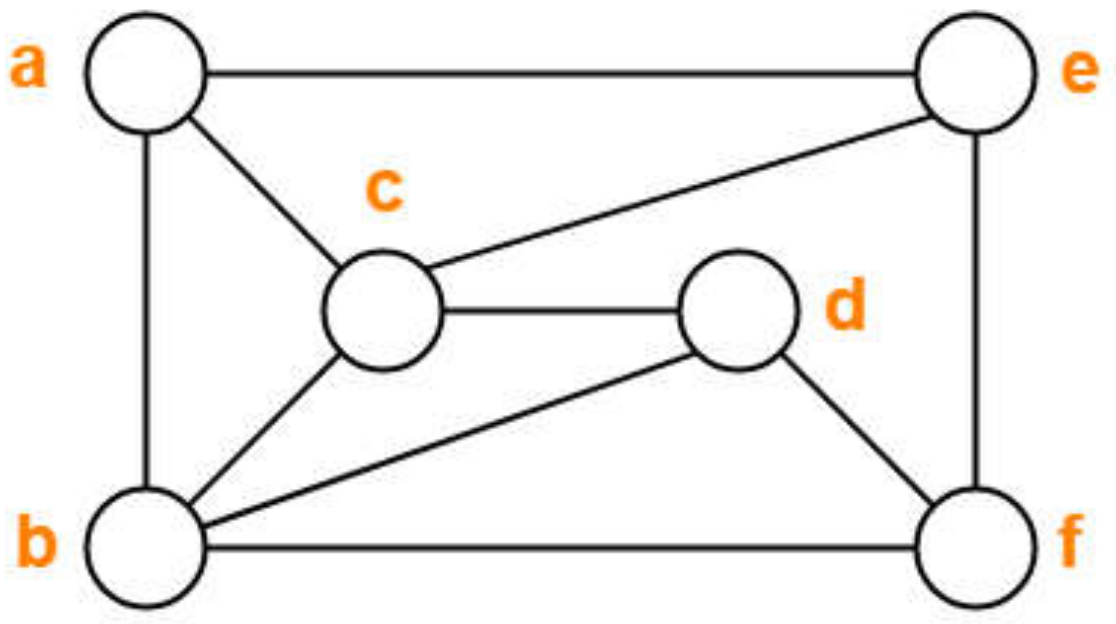
\includegraphics[scale=.15]{images/map-coloring}
		\end{figure}
		Posisi kandang dilambangkan dengan bulatan. Jika dua buah kandang dihubungkan oleh sebuah garis artinya ada jalan setapak yang menghubungkan secara langsung dua buah kandang tersebut. Seekor ayam tidak akan senang jika kandangnya berwarna sama dengan kandang ayam lain yang terhubung langsung dengan jalan setapak. 		
	\end{frame}

	\begin{frame}{Soal \#7 (2/2)}
		Karena dana yang terbatas, berapa minimal warna cat yang harus dibeli oleh Pak Blangkon sehingga semua ayam senang?
		\begin{description}
			\item[A.] 1
			\item[B.] 2
			\item[C.] 3
			\item[D.] 4
			\item[E.] 5
		\end{description}		
	\end{frame}

\section{Definisi Graf}
\begin{frame}{Definisi Graf}
	\begin{itemize}
		\item<2-> Graf terdiri atas \textbf{vertex} atau \textbf{simpul} atau \textbf{node} atau \textbf{titik}, (jamak: \textbf{vertices}) dan \textbf{sisi} atau \textbf{garis} yang disebut \textbf{edges}.		 
	\end{itemize}
	\begin{figure}[ht]
		\includegraphics<3->[scale=.25]{images/sifat-sifat-vertex-sisi}
	\end{figure}
\end{frame}

\begin{frame}{Terminology di Example 1.4.1~\citep{epp2020discrete} (1/2)}
	\begin{center}
		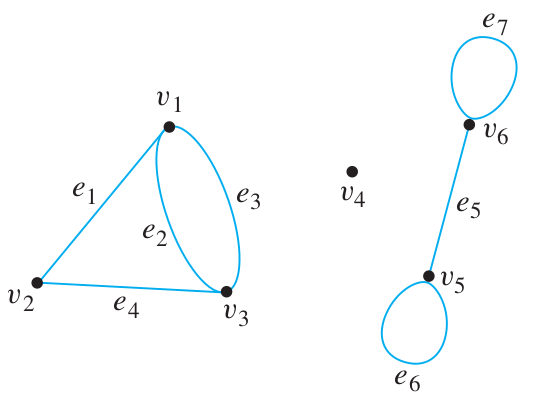
\includegraphics[scale=.25]{images/Example10-1-1}
	\end{center}
	\vspace*{-0.5cm}		
	\begin{itemize}
		\item<2-> Tuliskan semua himpunan simpul (\emph{vertex set}) dan himpunan sisi (\emph{edge set}), dan buatlah tabel yang menampilkan fungsi \emph{edge-endpoint}.
		\item<3-> Carilah semua sisi (\emph{edges}) yang bersinggungan dengan (\emph{incident}) $v_1$, semua simpul (\emph{vertices}) yang bertetangga dengan (\emph{adjacent}) $v_1$, semua sisi yang bertetangga (\emph{adjacent}) dengan $e_1$, semua \emph{loops}, semua \emph{parallel edges}, dan semua \emph{isolated vertices}.
	\end{itemize}
\end{frame}

\begin{frame}{Terminology di Example 1.4.1~\citep{epp2020discrete} (2/2)}
	\begin{itemize}
		\item<2-> vertex set = $\{ v_1, v_2, v_3, v_4, v_5, v_6 \}$ \\
		edge set = $\{ e_1, e_2, e_3, e_4, e_5, e_6, e_7 \}$ \\
		\begin{center}
			\includegraphics<3->[scale=.125]{images/fungsi-edge-to-point}				
		\end{center}
		\item<3-> $e_1$, $e_2$, and $e_3$ are incident on $v_1$. \\
		$v_2$ and $v_3$ are adjacent to $v_1$. \\
		$e_2$, $e_3$, and $e_4$ are adjacent to $e_1$. \\
		$e_6$ and $e_7$ are loops. \\
		$e_2$ and $e_3$ are parallel. \\
		$v_4$ is an isolated vertex. 		
	\end{itemize}
	
\end{frame}

\begin{frame}{Example 1.4.2~\citep{epp2020discrete}}
	Consider the graph specified as follows:
	\begin{center}
		vertex set = $\{ v_1, v_2, v_3, v_4 \}$ \\
		edge set = $\{ e_1, e_2, e_3, e_4 \}$
		
		\bigskip		
		
		edge-endpoint function:
	\end{center}
	\begin{center}
		\includegraphics<2->[scale=.25]{images/Example10-1-2}
	\end{center}
\end{frame}

\begin{frame}{Undirected and Directed Graph}
	\begin{itemize}
		\item<2-> A graph $G$ is called \textbf{undirected} if every edge in it is undirected.
		\item<3-> If a pair of vertices $(u, v)$ is not the same as the pair $(v, u)$, we say that the edge $(u, v)$ is \textbf{directed} from the vertex $u$, called the edge's \textbf{tail}, to the vertex v, called the edge's \textbf{head} \citep{levitin2012introduction}.
	\end{itemize}
	\begin{center}
		\includegraphics<4->[scale=.175]{images/directed-and-undirected}
	\end{center}
\end{frame}

\section{Konsep Derajat (Degree)}
\begin{frame}{Degree of the Vertex}
	\begin{block}{Definisi}
		\onslide<2->{Let $G$ be a graph and $v$ is a vertex of $G$.} \\
		\onslide<3->{The degree of $v$, denoted \textbf{deg($\bm{v}$)}, equals the number of edges that are incident on $v$, with an edge that is a loop counted twice.} \\
		\onslide<4->{The \textbf{total degree of $\bm{G}$} is the sum of the degrees of all the vertices of $G$.} 
	\end{block}
\end{frame}

\begin{frame}{Contoh Degree (1/2)}
	\begin{center}
		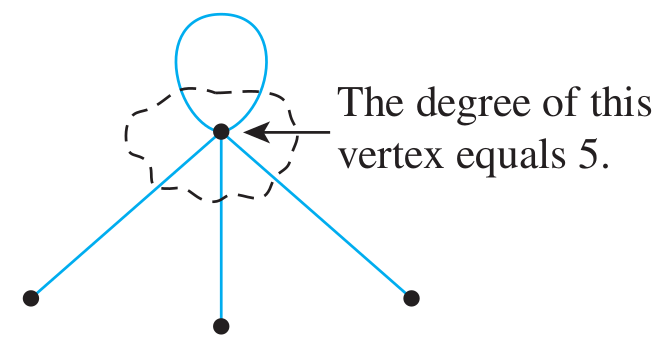
\includegraphics[scale=.3]{images/contoh-degree}
	\end{center}
\end{frame}

\begin{frame}{Contoh Degree (2/2)}
	Find the degree of each vertex of the graph $G$ shown below. Then find the total degree of $G$.
	\begin{center}
		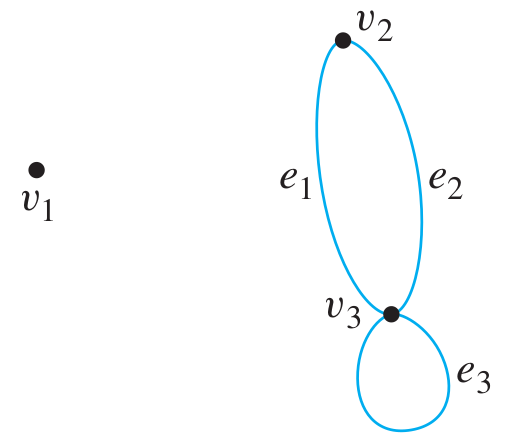
\includegraphics[scale=.25]{images/contoh-degree-2}
	\end{center}
\end{frame}

\begin{frame}{Using Graph to Color a Map (1/6)}
	Imagine that the diagram shown below is a map with countries labeled A-J~\citep{epp2020discrete}. \\
	Show that \textit{you can color the map so that no two adjacent countries have the same color}.	
	\begin{figure}[!ht]
		\centering
		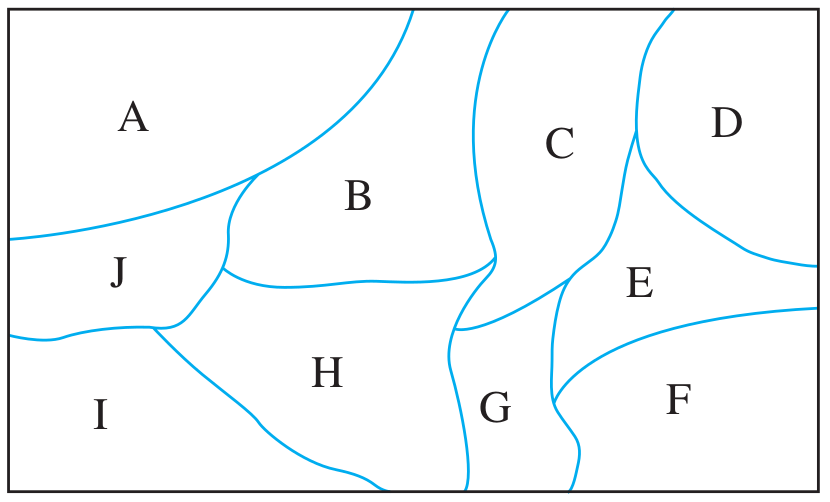
\includegraphics[scale=.25]{images/map-coloring-1}
	\end{figure}
\end{frame}

\begin{frame}{Using Graph to Color a Map (2/6)}
	To figure out a coloring, we can draw a graph, as shown below, where \textit{vertices represent countries} and where \textit{edges
		are drawn between pairs of vertices that represent adjacent countries}. \\
	\textit{\textbf{Coloring the vertices of the graph will translate to coloring the countries on the map}}.
	\begin{figure}[!ht]
		\centering
		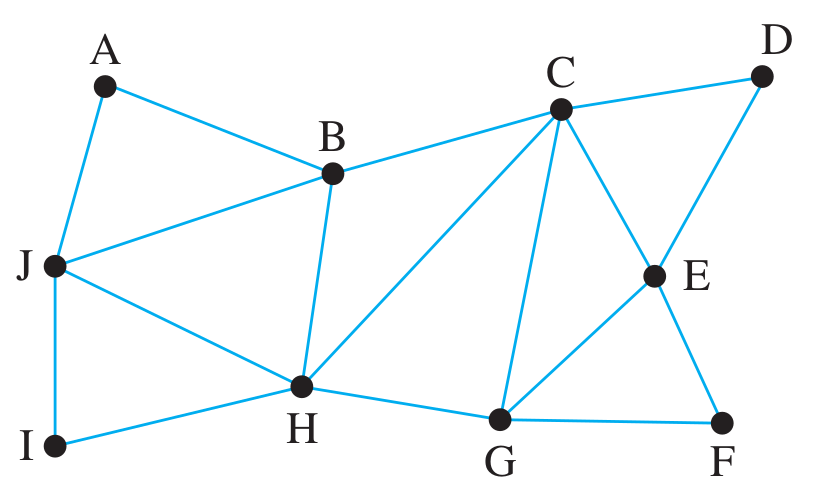
\includegraphics[scale=.25]{images/map-coloring-2}
	\end{figure}
\end{frame}

\begin{frame}{Using Graph to Color a Map (3/6)}
	\textbf{A relatively efficient strategy is}: \\
	At each stage, \textit{to focus on an uncolored vertex that has maximum degree}.
	\begin{figure}[!ht]
		\centering
		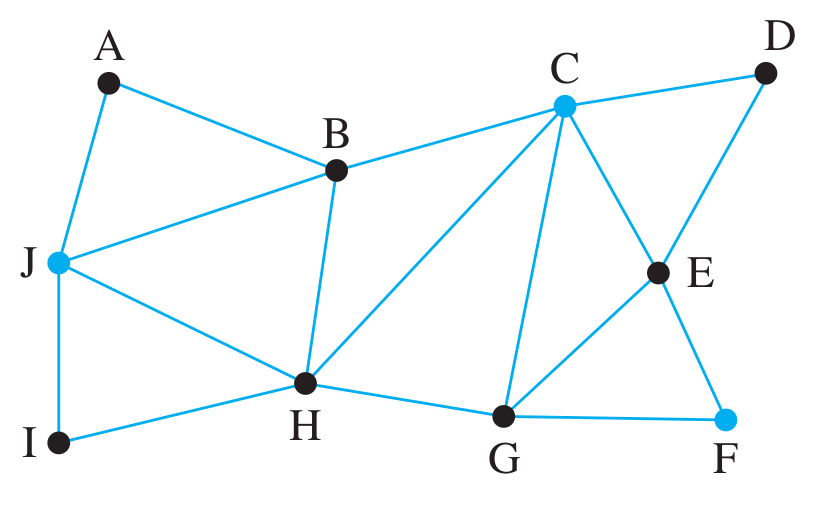
\includegraphics[scale=.25]{images/map-coloring-3}
	\end{figure}	
\end{frame}

\begin{frame}{Using Graph to Color a Map (4/6)}
	Since the vertices adjacent to C, J, and F cannot be colored blue, you can simplify the job of choosing additional colors by \textit{removing C, J, and F and the edges connecting them to adjacent vertices}.
	\begin{figure}[!ht]
		\centering
		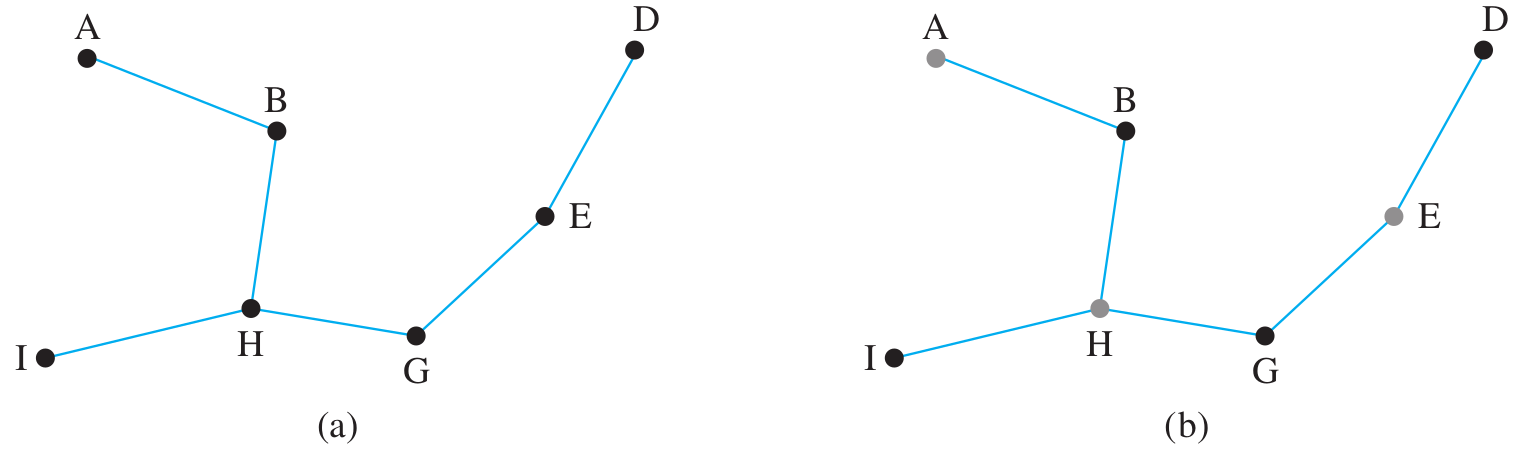
\includegraphics[scale=.2]{images/map-coloring-4}
	\end{figure}	
\end{frame}

\begin{frame}{Using Graph to Color a Map (5/6)}
	The drawing below shows the original graph with vertices C, J, and F colored \textbf{blue}, vertices H, A, and E, colored \textbf{gray}, and the
	remaining vertices colored \textbf{black}. \textit{You can check that no two adjacent vertices have the same color}.
	\begin{figure}[!ht]
		\centering
		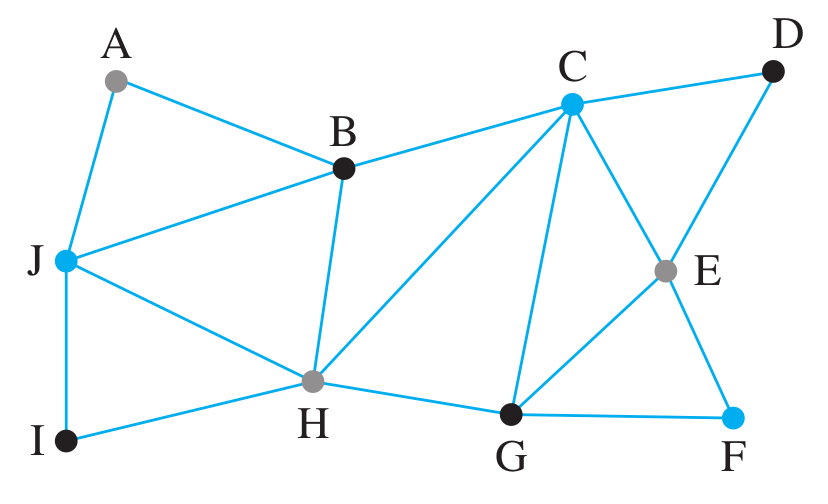
\includegraphics[scale=.25]{images/map-coloring-5}
	\end{figure}	
\end{frame}

\begin{frame}{Using Graph to Color a Map (6/6)}
	Translating the graph coloring back to the original map gives the following picture in which no two adjacent countries have the same color.
	\begin{figure}[!ht]
		\centering
		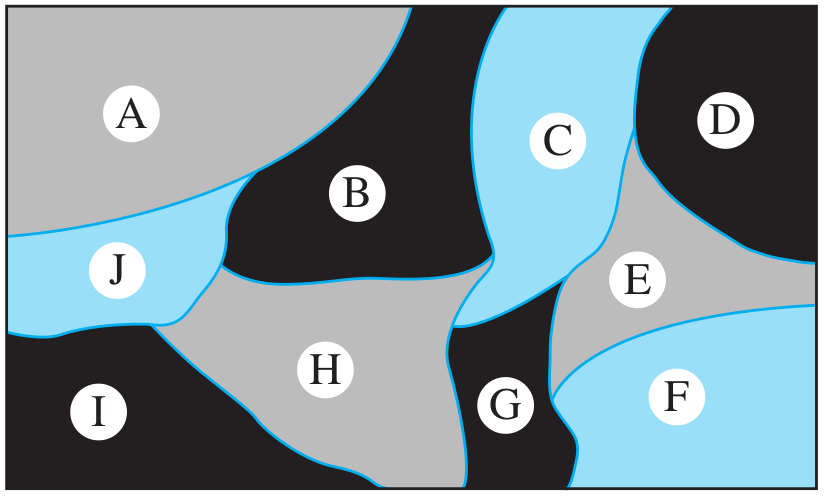
\includegraphics[scale=.25]{images/map-coloring-6}
	\end{figure}	
\end{frame}

	\begin{frame}{Kembali ke Soal \#7 (1/2)}
	Pak Blangkon berencana mengecat kandang-kandang ayamnya. Konfigurasi lokasi dari kandang yang dimiliki oleh Pak Blangkon adalah sebagai berikut:
	\begin{figure}[!ht]
		\centering
		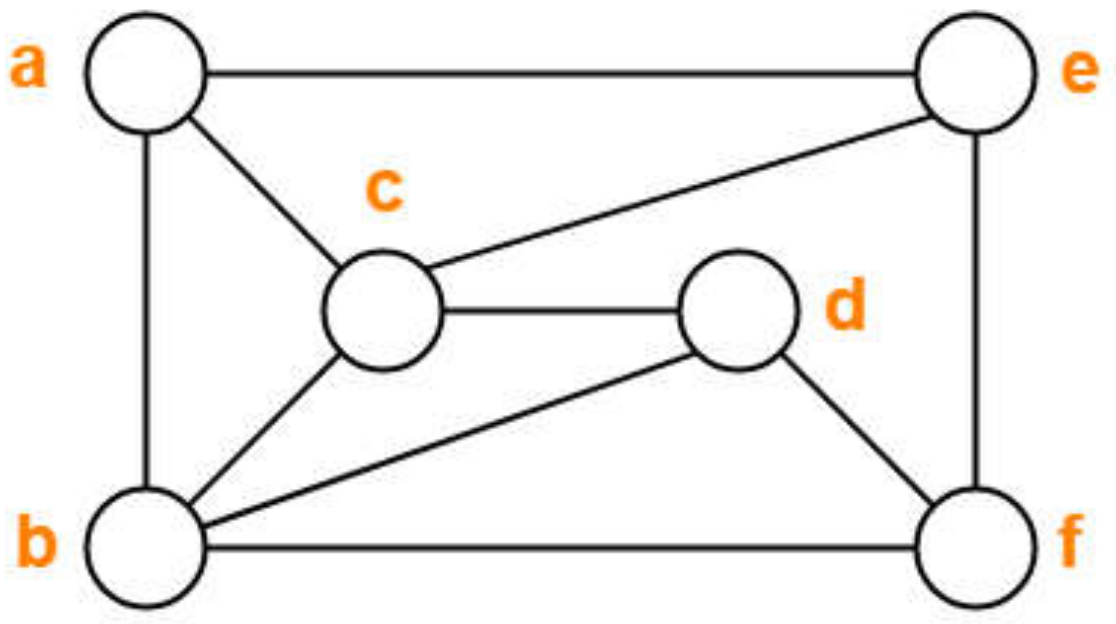
\includegraphics[scale=.15]{images/map-coloring}
	\end{figure}
	Posisi kandang dilambangkan dengan bulatan. Jika dua buah kandang dihubungkan oleh sebuah garis artinya ada jalan setapak yang menghubungkan secara langsung dua buah kandang tersebut. Seekor ayam tidak akan senang jika kandangnya berwarna sama dengan kandang ayam lain yang terhubung langsung dengan jalan setapak. 		
\end{frame}

\begin{frame}{Soal \#7 (2/2)}
	Karena dana yang terbatas, berapa minimal warna cat yang harus dibeli oleh Pak Blangkon sehingga semua ayam senang?
	\begin{description}
		\item[A.] 1
		\item[B.] 2
		\item[C.] 3
		\item[D.] 4
		\item[E.] 5
	\end{description}		
	\pause \textbf{Jawab: C}	
\end{frame}


	\begin{frame}{Soal \#8 (1/2)}
		Terdapat 15 pengguna facebook yaitu $A$, $B$, $C$, $D$, $E$, $F$, $G$, $H$, $I$, $J$, $K$, $L$, $M$, $N$, dan $O$. Fungsi pertemanan $F(X,Y)$ menyatakan bahwa $X$ dan $Y$ berteman di Facebook. Jika $X$ dan $Y$ berteman kemudian $Y$ dan $Z$ berteman, maka bisa dipastikan bahwa $X$, $Y$, dan $Z$ berada pada lingkaran pertemanan yang sama. Anda diberikan informasi status pertemanan antara pengguna sebagai berikut:
		\begin{table}[!ht]
			\centering
			\begin{tabular}{|l|l|l|}
				\hline
				$F(A,B)$ & $F(C,M)$ & $F(E,G)$ \\
				\hline
				$F(A,D)$ & $F(D,J)$ & $F(O,N)$ \\
				\hline
				$F(A,O)$ & $F(K,L)$ & $F(D,C)$ \\
				\hline
				$F(B,N)$ & $F(L,H)$ & $F(H,I)$ \\
				\hline
			\end{tabular}
		\end{table}
	\end{frame}

	\begin{frame}{Soal \#8 (2/2)}
	Berapakah banyaknya lingkaran pertemanan yang terbentuk?
	\begin{description}
		\item[A.] 1
		\item[B.] 2
		\item[C.] 3
		\item[D.] 4
		\item[E.] 5
	\end{description}		
	\pause \textbf{Jawab: C}	
	\end{frame}

	\begin{frame}{Soal \#9 (1/2)}
		Bebek-bebek baru Pak Dengklek yang bernama Anto, Budi, Candra, Doni, Eko, Ferdi, Geri, Hendra, Igor, dan Joko belum saling mengenal satu sama lain. Definisi \textit{saling mengenal} adalah \textit{bebek A mengenal bebek B jika dan hanya jika bebek B mengenal bebek A juga}. Berikut adalah daftar bebek-bebek yang telah dikenal oleh masing-masing bebek.
		
		\bigskip
		\begin{tabular}{ll}
			Anto      &: Eko, Doni, dan Ferdi \\
			Budi      &: Anto, Hendra, Joko, Eko, dan Ferdi \\
			Candra    &: Ferdi, Hendra, dan Joko \\
			Doni      &: Anto, Candra, dan Budi \\
			Eko       &: Joko, Igor, Hendra, Budi, dan Anto \\
			Ferdi     &: Hendra, Igor, Geri, Anto, dan Budi \\
			Geri      &: Anto, Budi, Ferdi, dan Joko \\
			Hendra    &: Anto, Eko, Ferdi, Igor, Joko, dan Budi \\
			Igor      &: Geri, Hendra, Joko, Eko, dan Ferdi \\
			Joko      &: Igor, Hendra, Anto, Geri, Eko, dan Budi
		\end{tabular} 
	\end{frame}


	\begin{frame}{Soal \#9 (2/2)}
		Suatu hari Pak Dengklek ingin bertamasya bersama bebek-bebeknya menggunakan beberapa mobil. Setiap mobil hanya boleh diisi oleh bebek-bebek yang sudah saling mengenal saja. Berapakah mobil minimum yang harus disiapkan Pak Dengklek?
		\begin{description}
			\item[A.] 1
			\item[B.] 3
			\item[C.] 4
			\item[D.] 5
			\item[E.] 8
		\end{description}		
		\pause \textbf{Jawab: D}	
	\end{frame}

	\begin{frame}{Soal \#10 (1/2)}
		Pak Dengklek merupakan ilmuwan terbaik di Singanesia. Saat ini ia hendak mencoba penemuan terbarunya, mesin teleportasi! Ia ingin mencoba mesinnya tersebut untuk memindahkan barang sejauh mungkin. Untungnya, Singanesia merupakan negara yang cukup besar.
		\begin{figure}[!ht]
			\centering
			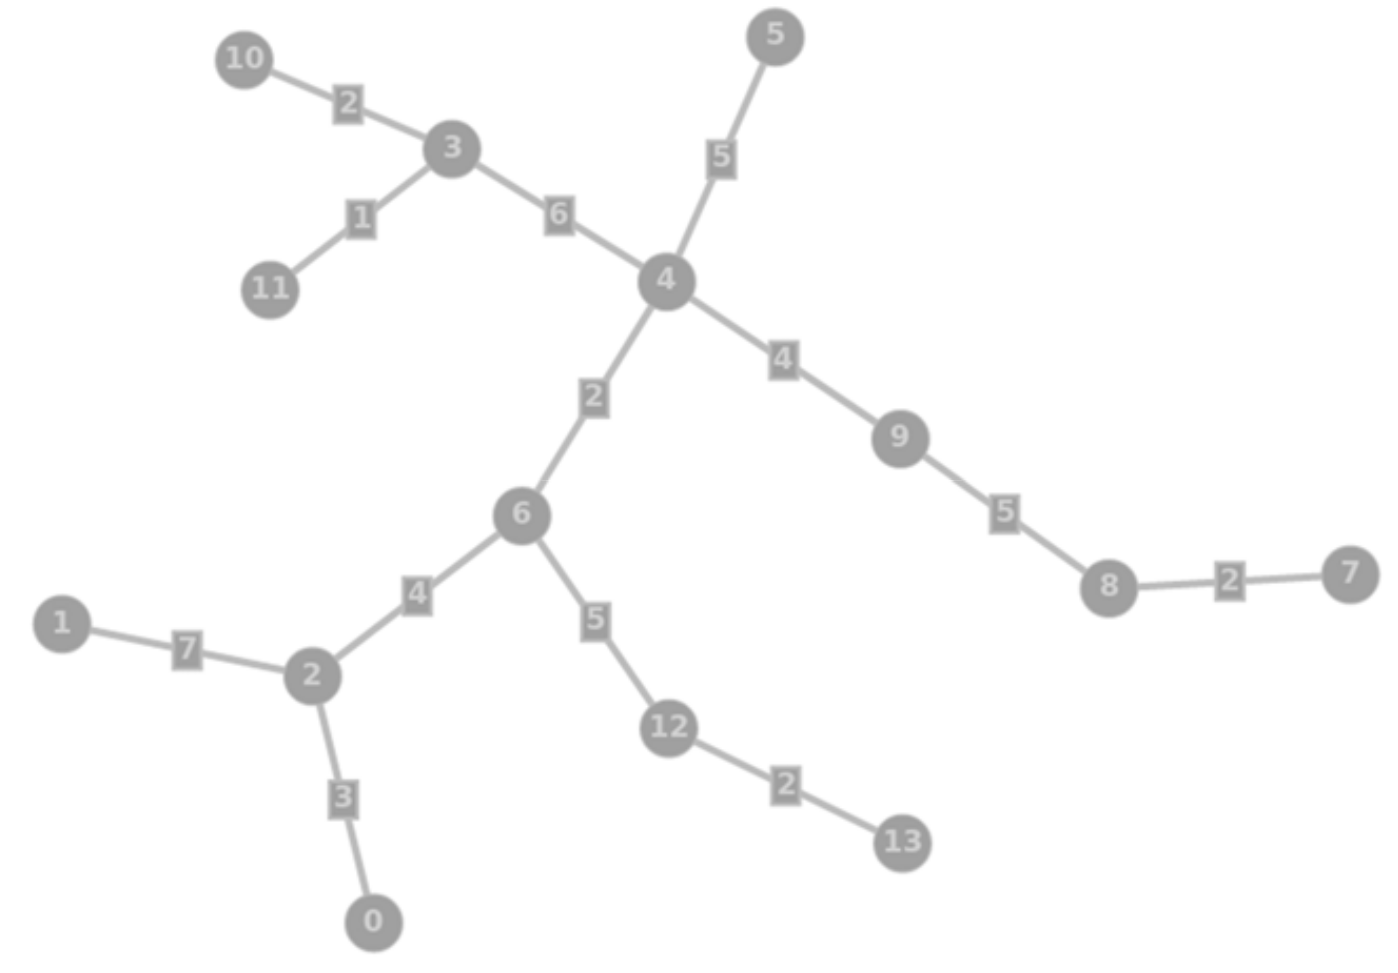
\includegraphics[scale=.1675]{images/singanesia}
		\end{figure}

	\end{frame}
	
\begin{frame}{Soal \#10 (2/2)}
	Bantulah Pak Dengklek mencari pasangan kota terjauh yang mungkin! Perhatikan bahwa pasangan kota terjauh yang dimaksud adalah 
	2 buah kota $A$ dan $B$ sedemikian sehingga untuk \textit{setiap pasangan kota} $C$ dan $D$, $C \neq A$ atau $D \neq B$, jarak dari kota $A$ dan $B$ di graf di atas lebih besar daripada jarak $C$ dan $D$.
		\begin{description}
	\item[A.] 22
	\item[B.] 23
	\item[C.] 24
	\item[D.] 25
	\item[E.] 26
\end{description}		
\end{frame}

\begin{frame}{Graph Representations}
	Graphs for computer algorithms are usually represented in one of two ways \citep{levitin2012introduction}: 
	\begin{itemize}
		\item<2-> the adjacency matrix and
		\item<3-> adjacency lists.
	\end{itemize}  
\end{frame}

\begin{frame}{\textit{The Adjacency Matrix} (Matriks Ketetanggaan)}
	The \textit{adjacency matrix} of a graph with $n$ vertices is an $n \times n$ boolean matrix with one row and one column for each of the graph's vertices, in which the element in the $i$th row and the $j$th column is equal to $1$ if there is an edge from the $i$th vertex to the $j$th vertex, and equal to $0$ if there is no such edge \citep{levitin2012introduction}.
	
	\begin{center}
		\includegraphics<2->[scale=.125]{images/graf-contoh} \; \includegraphics<3->[scale=.125]{images/adjacency-matrix-contoh}
	\end{center}
	\onslide<4->{Note that the adjacency matrix of an undirected graph is always symmetric, i.e., $A[i, j ] = A[j, i]$ for every $0 \leq i$, $j \leq n - 1$ (why?).}
\end{frame}

\begin{frame}{\textit{The Adjacency Lists}}
	The adjacency lists of a graph is a collection of linked lists, one for each vertex, that contain all the vertices adjacent to the list's vertex (i.e., all the vertices connected to it by an edge) \citep{levitin2012introduction}.
	\begin{center}
	\includegraphics<2->[scale=.1]{images/graf-contoh} \; \includegraphics<3->[scale=.1]{images/adjacency-list-contoh}
\end{center}
\onslide<4->{If a graph is sparse, the adjacency list representation may use less space than the corresponding adjacency matrix; the situation is exactly opposite for dense graphs. In general, which of the two representations is more convenient depends on the nature of the problem, on the algorithm used for solving it, and, possibly, on the type of input graph (sparse or dense).}
\end{frame}

\begin{frame}{\textit{Weighted Graphs}}
	\onslide<2->{A weighted graph is a graph with \textbf{numbers} assigned to its edges. These numbers are called \textbf{weights} or \textbf{costs} \citep{levitin2012introduction}. An interest in such graphs is motivated by numerous real-world applications, such as} 
	\begin{itemize}
		\item<3-> finding the shortest path between two points in a transportation or
		\item<4-> communication network or the traveling salesman problem mentioned earlier.
	\end{itemize}
	\begin{center}
		\includegraphics<5->[scale=.2]{images/weighted-graph-contoh}
	\end{center}	
\end{frame}

\begin{frame}{Floyd's Algorithm (All-Pairs Shortest-Paths Problem)}
	\begin{itemize}
		\item<2-> Given a weighted connected graph (undirected or directed), the all-pairs shortest-paths problem asks to ?nd the distances -- i.e., the lengths of the shortest paths -- from each vertex to all other vertices.
		\item<3-> This is one of several variations of the problem involving shortest paths in graphs.
		\item<4-> Because of its important applications to \textbf{communications}, \textbf{transportation networks}, and \textbf{operations research}, it has been thoroughly studied over the years. 
		\item<5-> Among recent applications of the all-pairs shortest-path problem is precomputing distances for motion planning in computer games. 
		\item<6-> It is convenient to record the lengths of shortest paths in an $n \times n$ matrix $D$ called the \textbf{distance matrix}: the element $d_{ij}$ in the $i$th row and the $j$th column of this matrix indicates the length of the shortest path from the $i$th vertex to the $j$th vertex \citep{levitin2012introduction}.		
	\end{itemize}	
\end{frame}

\begin{frame}{\textit{Distance Matrix}}
	\begin{center}
		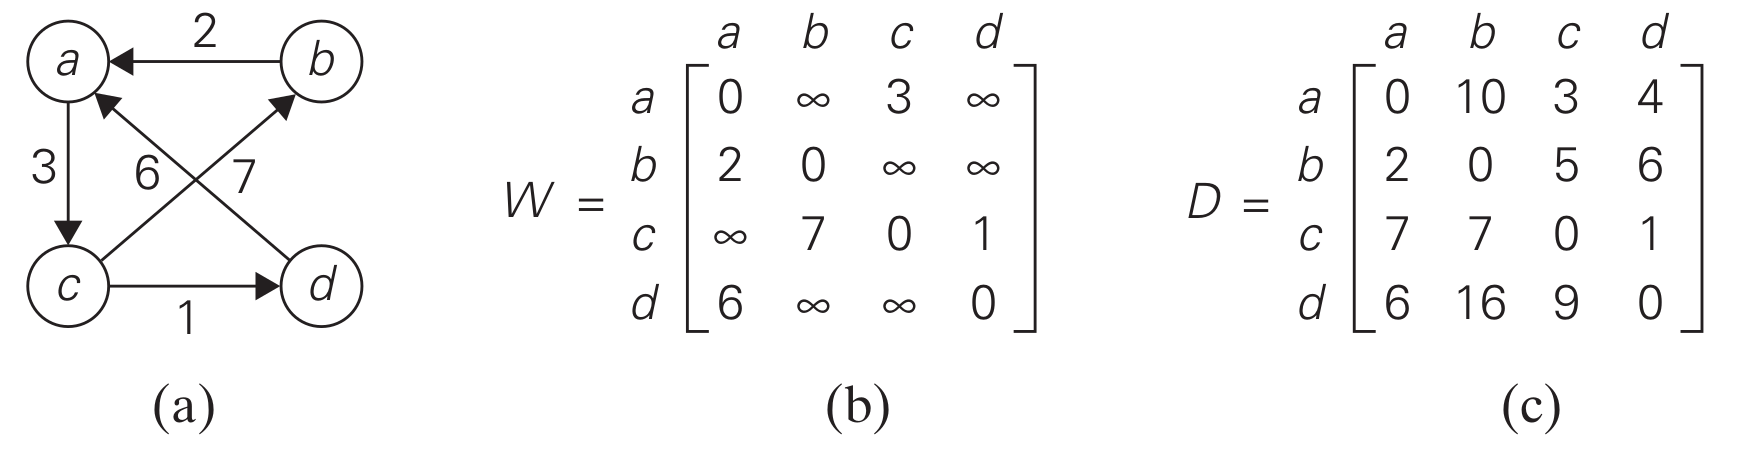
\includegraphics[scale=.185]{images/distance-matrix}
	\end{center}
	\begin{description}
	\item<2->[(a)] Directed graph
	\item<3->[(b)] Its weight matrix
	\item<4->[(c)] Its distance matrix
	\end{description}		
\end{frame}

\begin{frame}{Floyd's Algorithm (All-Pairs Shortest-Paths Problem)}
	\begin{center}
		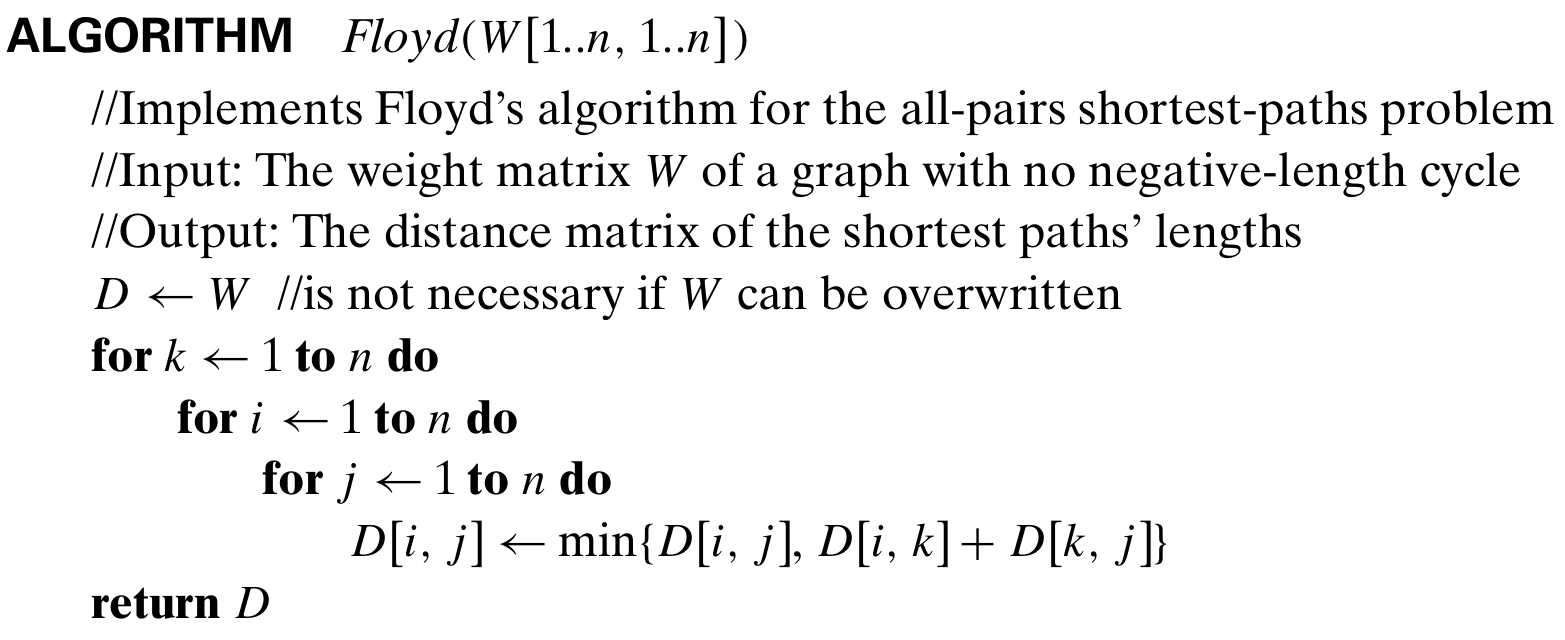
\includegraphics[scale=.21]{images/floyd-algorithm}
	\end{center}
\end{frame}

\begin{frame}{Contoh Floyd's Algorithm}
	\begin{center}
		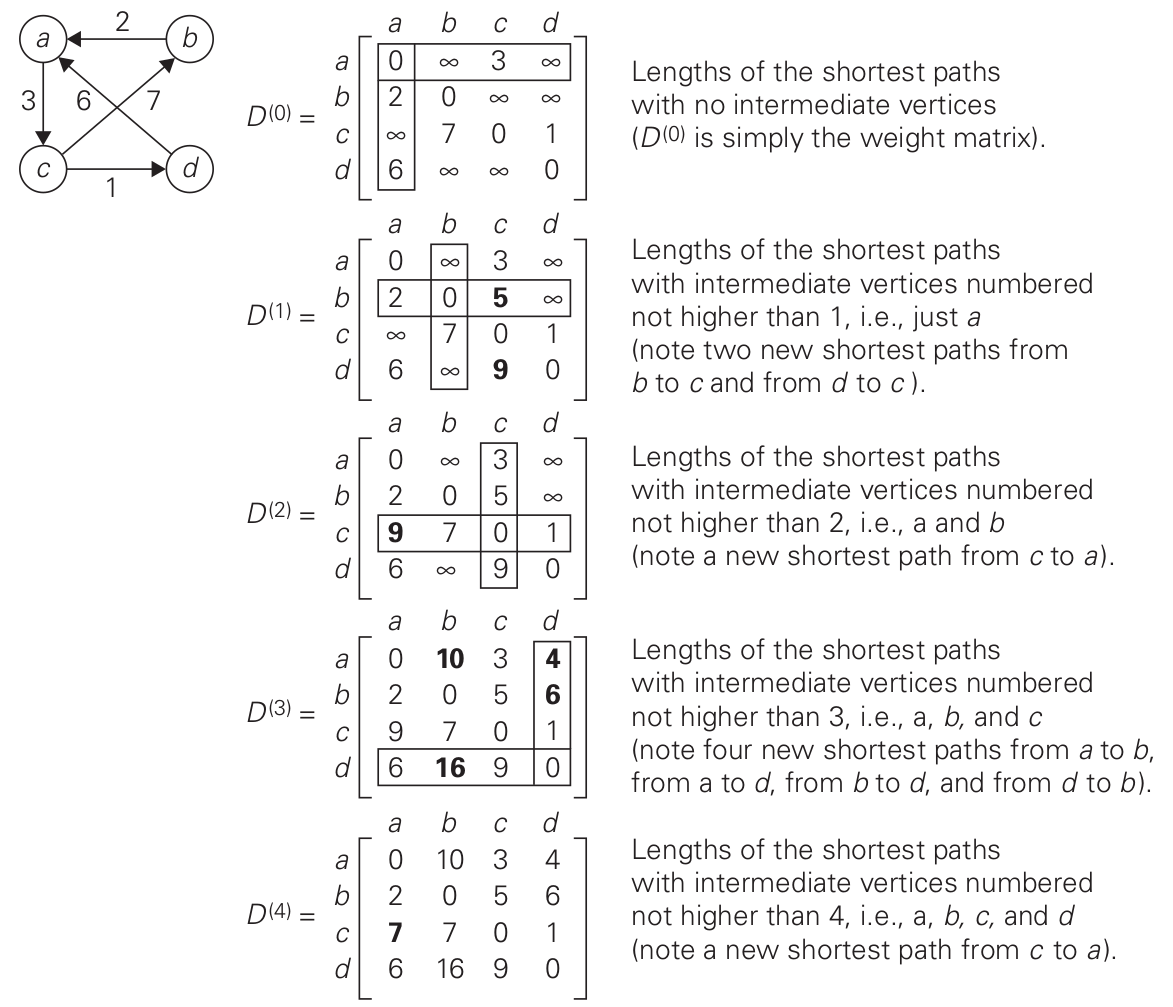
\includegraphics[scale=.24]{images/floyd-algorithm-example}
	\end{center}
\end{frame}

\begin{frame}{Kembali ke Soal \#10 (1/2)}
	Pak Dengklek merupakan ilmuwan terbaik di Singanesia. Saat ini ia hendak mencoba penemuan terbarunya, mesin teleportasi! Ia ingin mencoba mesinnya tersebut untuk memindahkan barang sejauh mungkin. Untungnya, Singanesia merupakan negara yang cukup besar.
	\begin{figure}[!ht]
		\centering
		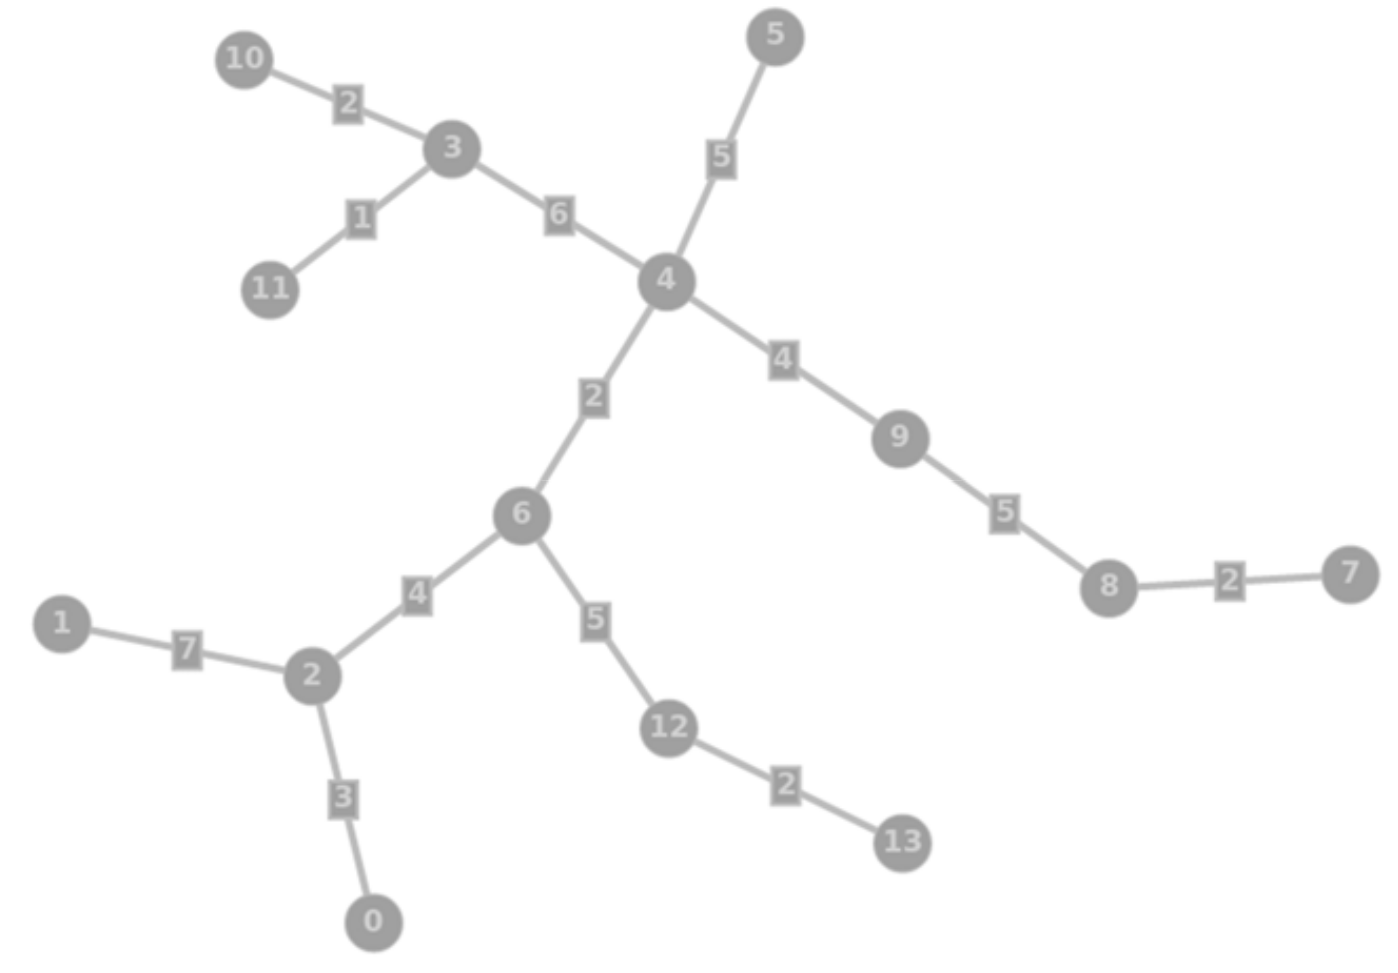
\includegraphics[scale=.1675]{images/singanesia}
	\end{figure}
	
\end{frame}

\begin{frame}{Soal \#10 (2/2)}
	Bantulah Pak Dengklek mencari pasangan kota terjauh yang mungkin! Perhatikan bahwa pasangan kota terjauh yang dimaksud adalah 
	2 buah kota $A$ dan $B$ sedemikian sehingga untuk \textit{setiap pasangan kota} $C$ dan $D$, $C \neq A$ atau $D \neq B$, jarak dari kota $A$ dan $B$ di graf di atas lebih besar daripada jarak $C$ dan $D$.
	\begin{description}
		\item[A.] 22
		\item[B.] 23
		\item[C.] 24
		\item[D.] 25
		\item[E.] 26
	\end{description}		
	\pause \textbf{Jawab: C}		
\end{frame}

	%%%% predictive distribution
	
	
	% \begin{frame}
		%   \frametitle{Some other one parameter models}
		
		%   \begin{itemize}
			%   \item Poisson
			%   \item Exponential
			%   \item Cauchy
			%   \end{itemize}
		
		% \end{frame}
	
	\section<presentation>*{\appendixname}
	\subsection<presentation>*{For Further Reading}
	
	\begin{frame}[allowframebreaks]
		\frametitle<presentation>{Daftar Pustaka}
		{\footnotesize
			%    \bibliographystyle{apalike}
			\bibliography{references}
		}    
	\end{frame}
	
\end{document}

%%% Local Variables: 
%%% TeX-PDF-mode: t
%%% TeX-master: t
%%% End: 
